%%
%% This is file `sample-manuscript.tex',
%% generated with the docstrip utility.
%%
%% The original source files were:
%%
%% samples.dtx  (with options: `manuscript')
%% 
%% IMPORTANT NOTICE:
%% 
%% For the copyright see the source file.
%% 
%% Any modified versions of this file must be renamed
%% with new filenames distinct from sample-manuscript.tex.
%% 
%% For distribution of the original source see the terms
%% for copying and modification in the file samples.dtx.
%% 
%% This generated file may be distributed as long as the
%% original source files, as listed above, are part of the
%% same distribution. (The sources need not necessarily be
%% in the same archive or directory.)
%%
%% Commands for TeXCount
%TC:macro \cite [option:text,text]
%TC:macro \citep [option:text,text]
%TC:macro \citet [option:text,text]
%TC:envir table 0 1
%TC:envir table* 0 1
%TC:envir tabular [ignore] word
%TC:envir displaymath 0 word
%TC:envir math 0 word
%TC:envir comment 0 0
%%
%%
%% The first command in your LaTeX source must be the \documentclass command.
%%%% Small single column format, used for CIE, CSUR, DTRAP, JACM, JDIQ, JEA, JERIC, JETC, PACMCGIT, TAAS, TACCESS, TACO, TALG, TALLIP (formerly TALIP), TCPS, TDSCI, TEAC, TECS, TELO, THRI, TIIS, TIOT, TISSEC, TIST, TKDD, TMIS, TOCE, TOCHI, TOCL, TOCS, TOCT, TODAES, TODS, TOIS, TOIT, TOMACS, TOMM (formerly TOMCCAP), TOMPECS, TOMS, TOPC, TOPLAS, TOPS, TOS, TOSEM, TOSN, TQC, TRETS, TSAS, TSC, TSLP, TWEB.
% \documentclass[acmsmall]{acmart}

%%%% Large single column format, used for IMWUT, JOCCH, PACMPL, POMACS, TAP, PACMHCI
% \documentclass[acmlarge,screen]{acmart}

%%%% Large double column format, used for TOG
% \documentclass[acmtog, authorversion]{acmart}

%%%% Generic manuscript mode, required for submission
%%%% and peer review
\documentclass[manuscript,screen,review]{acmart}
%% Fonts used in the template cannot be substituted; margin 
%% adjustments are not allowed.
%%
%% \BibTeX command to typeset BibTeX logo in the docs
\AtBeginDocument{%
  \providecommand\BibTeX{{%
    \normalfont B\kern-0.5em{\scshape i\kern-0.25em b}\kern-0.8em\TeX}}}

%% Rights management information.  This information is sent to you
%% when you complete the rights form.  These commands have SAMPLE
%% values in them; it is your responsibility as an author to replace
%% the commands and values with those provided to you when you
%% complete the rights form.
\setcopyright{acmcopyright}
\copyrightyear{2018}
\acmYear{2018}
\acmDOI{XXXXXXX.XXXXXXX}

%% These commands are for a PROCEEDINGS abstract or paper.
\acmConference[Conference acronym 'XX]{Make sure to enter the correct
  conference title from your rights confirmation emai}{June 03--05,
  2018}{Woodstock, NY}
%
%  Uncomment \acmBooktitle if th title of the proceedings is different
%  from ``Proceedings of ...''!
%
\acmBooktitle{Woodstock '18: ACM Symposium on Neural Gaze Detection,
 June 03--05, 2018, Woodstock, NY} 
\acmPrice{15.00}
\acmISBN{978-1-4503-XXXX-X/18/06}


%%
%% Submission ID.
%% Use this when submitting an article to a sponsored event. You'll
%% receive a unique submission ID from the organizers
%% of the event, and this ID should be used as the parameter to this command.
%%\acmSubmissionID{123-A56-BU3}

%%
%% For managing citations, it is recommended to use bibliography
%% files in BibTeX format.
%%
%% You can then either use BibTeX with the ACM-Reference-Format style,
%% or BibLaTeX with the acmnumeric or acmauthoryear sytles, that include
%% support for advanced citation of software artefact from the
%% biblatex-software package, also separately available on CTAN.
%%
%% Look at the sample-*-biblatex.tex files for templates showcasing
%% the biblatex styles.
%%

%%
%% The majority of ACM publications use numbered citations and
%% references.  The command \citestyle{authoryear} switches to the
%% "author year" style.
%%
%% If you are preparing content for an event
%% sponsored by ACM SIGGRAPH, you must use the "author year" style of
%% citations and references.
%% Uncommenting
%% the next command will enable that style.
%%\citestyle{acmauthoryear}

%%
%% end of the preamble, start of the body of the document source.
\begin{document}

\title{Task 3  Numerical Methods}
\author{Carl-Emil Rohde \\ kvb125@alumni.ku.dk}
\date{September 2023}

\maketitle

\section*{Problem 1}

\subsection*{5.2.30}
I can use the Gershgorin Circle Theorem to define disks in which the eigenvalues $\lambda$ of $A$ must lie. For each row $i$, I create a disk $D_i$ centered at the diagonal entry $a_{i i}$ with a radius $R_i=\sum_{j \neq i}\left|a_{i j}\right|$:
\\
\textbf{$D_1$} is centered at 6 with radius $R_1=2+1=3$. Therefore, $D_1$ gives us $3 \leq|\lambda-6|$, leading to $3 \leq|\lambda| \leq 9$.
\\
\textbf{$D_2$} is centered at -5 with radius $R_2=1+0=1$. Therefore, $D_2$ gives us $1 \leq|\lambda+5|$, leading to $4 \leq|\lambda| \leq 6$.
\\
\textbf{$D_3$} is centered at 4 with radius $R_3=2+1=3$. Therefore, $D_3$ gives us $1 \leq|\lambda-4|$, leading to $1 \leq|\lambda| \leq 7$.
\\
By the Gershgorin Circle Theorem, all eigenvalues must lie within at least one of these disks. The intersection of these regions is $1 \leq|\lambda| \leq 9$, confirming that all eigenvalues of $A$ must satisfy this inequality.

\subsection*{5.2.37}
\textbf{Sketch the Gershgorin disks.}
\\
For the given matrix $A$,
$$
A=\left[\begin{array}{rrr}
0 & 2 & -1 \\
-2 & -10 & 0 \\
-1 & -1 & 4
\end{array}\right]
$$
I can apply the Gershgorin Circle Theorem to find the Gershgorin disks.
\\
\\
The first disk \textbf{$D_1$} is centered at 0 with radius $R_1=2+1=3$. Therefore, $D_1: \mid \lambda-$ $0|\leq 3 \Rightarrow| \lambda \mid \leq 3$.
\\
The second disk \textbf{$D_2$} is centered at -10 with radius $R_2=2+0=2$. Therefore, $D_2: \mid \lambda+$ $10|\leq 2 \Rightarrow 8 \leq| \lambda \mid \leq 12$.
\\
The third disk \textbf{$D_3$} is centered at 4 with radius $R_3=1+1=2$. Therefore, $D_3: \mid \lambda-$ $4|\leq 2 \Rightarrow 2 \leq| \lambda \mid \leq 6$.
\\
\\
Using the Gershgorin Circle Theorem, every eigenvalue $\lambda$ of $A$ must lie within at least one of these disks. The widest range for $|\lambda|$ is $[2,12]$.
\\
\\
\textbf{Bound for Spectral Radius}
From Theorem 4 in the text book:,
$$
\rho(A)=\inf _{\|\cdot\|}\|A\|
$$
I know $\rho(A)$ is the infimum of all subordinate matrix norms of $A$.
\\
Since I am provided the $\|\cdot\|_{\infty}$ matrix norm as defined by
$$
\|A\|_{\infty}=\max _{1 \leq i \leq n} \sum_{j=1}^n\left|a_{i j}\right|
$$
I can easily find this norm for $A$ :
$$
\|A\|_{\infty}=\max \{3,12,6\}=12
$$
By Theorem 4, $\rho(A) \leq\|A\|_{\infty}=12$.
\\
However, I already know from the Gershgorin disks that $\rho(A)$ must be in the range $[2,12]$ . Therefore, the bound for $\rho(A)$ is $2 \leq \rho(A) \leq 12$.

\subsection*{5.3.30}
To find the least-squares solution, I will use the QR factorization method as hinted.
I start by rewriting the problem in matrix form $A X=B$, where
$$
A=\left(\begin{array}{ll}
3 & 2 \\
2 & 3 \\
1 & 2
\end{array}\right), \quad X=\left(\begin{array}{l}
x \\
y
\end{array}\right), \quad B=\left(\begin{array}{l}
3 \\
0 \\
1
\end{array}\right)
$$
I'll first find the QR factorization of matrix $A$. $A$ can be factored into $Q$ and $R$ where $Q$ is an orthogonal matrix and $R$ is an upper triangular matrix. I have used python for these calculations. 
\\
\\
Based on the content from page 279 , the least-squares solution $X$ can be computed as:
$$
X=R^{-1} Q^T B
$$
This I have implemented in python using the np.linalg.qr method. 
\\
\\
Upon running this code, I get:
$$
X=[1.38095238,-0.66666667]
$$
Therefore, the least-squares solution to the given system is $x=1.38095238$ and $y=$ -0.66666667.

\subsection*{5.4.1}
\textbf{1. Matrix A} $=\left[\begin{array}{ccc}4 & 0 & 0 \\ 0 & 0 & 0 \\ 0 & 0 & 7 \\ 0 & 0 & 0\end{array}\right]$
\\
\\
Firstly, $$A^* A=\left[\begin{array}{lll}16 & 0 & 0 \\ 0 & 0 & 0 \\ 0 & 0 & 49\end{array}\right]$$
\\
The eigenvalues are $\sigma_1^2=49, \sigma_2^2=16, \sigma_3^2=0$, so $\sigma_1=7, \sigma_2=4, \sigma_3=0$.
\\
I can choose the unitary matrix $Q$ as an identity matrix $I$ because $A^* A$ is already diagonal.
$Q=\left[\begin{array}{lll}1 & 0 & 0 \\ 0 & 1 & 0 \\ 0 & 0 & 1\end{array}\right]$
\\
Matrix $P$ can also be chosen as an identity matrix $I$.
$P=\left[\begin{array}{llll}1 & 0 & 0 & 0 \\ 0 & 1 & 0 & 0 \\ 0 & 0 & 1 & 0 \\ 0 & 0 & 0 & 1\end{array}\right]$
\\
Matrix $D$ will then be:
$D=\left[\begin{array}{lll}7 & 0 & 0 \\ 0 & 4 & 0 \\ 0 & 0 & 0 \\ 0 & 0 & 0\end{array}\right]$
\\
\\
\textbf{2. Matrix B}$=\left[\begin{array}{ll}2 & 1\end{array}\right]$
$$
B^* B=\left[\begin{array}{ll}
4 & 2 \\
2 & 1
\end{array}\right]
$$
Eigenvalues are $\sigma_1^2=5, \sigma_2^2=0$, so $\sigma_1=\sqrt{5}, \sigma_2=0$.
Let's take
$$
Q=\left[\begin{array}{ll}
\frac{1}{\sqrt{5}} & -\frac{2}{\sqrt{5}} \\
\frac{2}{\sqrt{5}} & \frac{1}{\sqrt{5}}
\end{array}\right]
$$
Since $B$ is $1 \times 2, P$ will be a $1 \times 1$ identity matrix, and $D$ will be:
$$
D=\left[\begin{array}{ll}
\sqrt{5} & 0
\end{array}\right]
$$
\\
\\
\textbf{3. Matrix C}$=\left[\begin{array}{r}5 \\ -4\end{array}\right]$
$$
C^* C=[25+16]=41
$$
Eigenvalue $\sigma_1^2=41$, so $\sigma_1=\sqrt{41}$.
\\
\\
Here $P$ will be a $2 \times 2$ identity matrix, $Q$ will be a $1 \times 1$ identity matrix, and $D$ will be:
$$
D=[\sqrt{41}]
$$
I have now found the SVDs for all three matrices.
\section*{Problem 2}
 To solve this problem I have implemented the Power method for each given matrix $A$ and initial vector $x_0$. I have then plotted the estimated dominant eigenvalue, $r$, as a function of iterations (up to 100 iterations). I have done all of this in Python. Below are the results and an explanation for each case:
 \begin{center}
    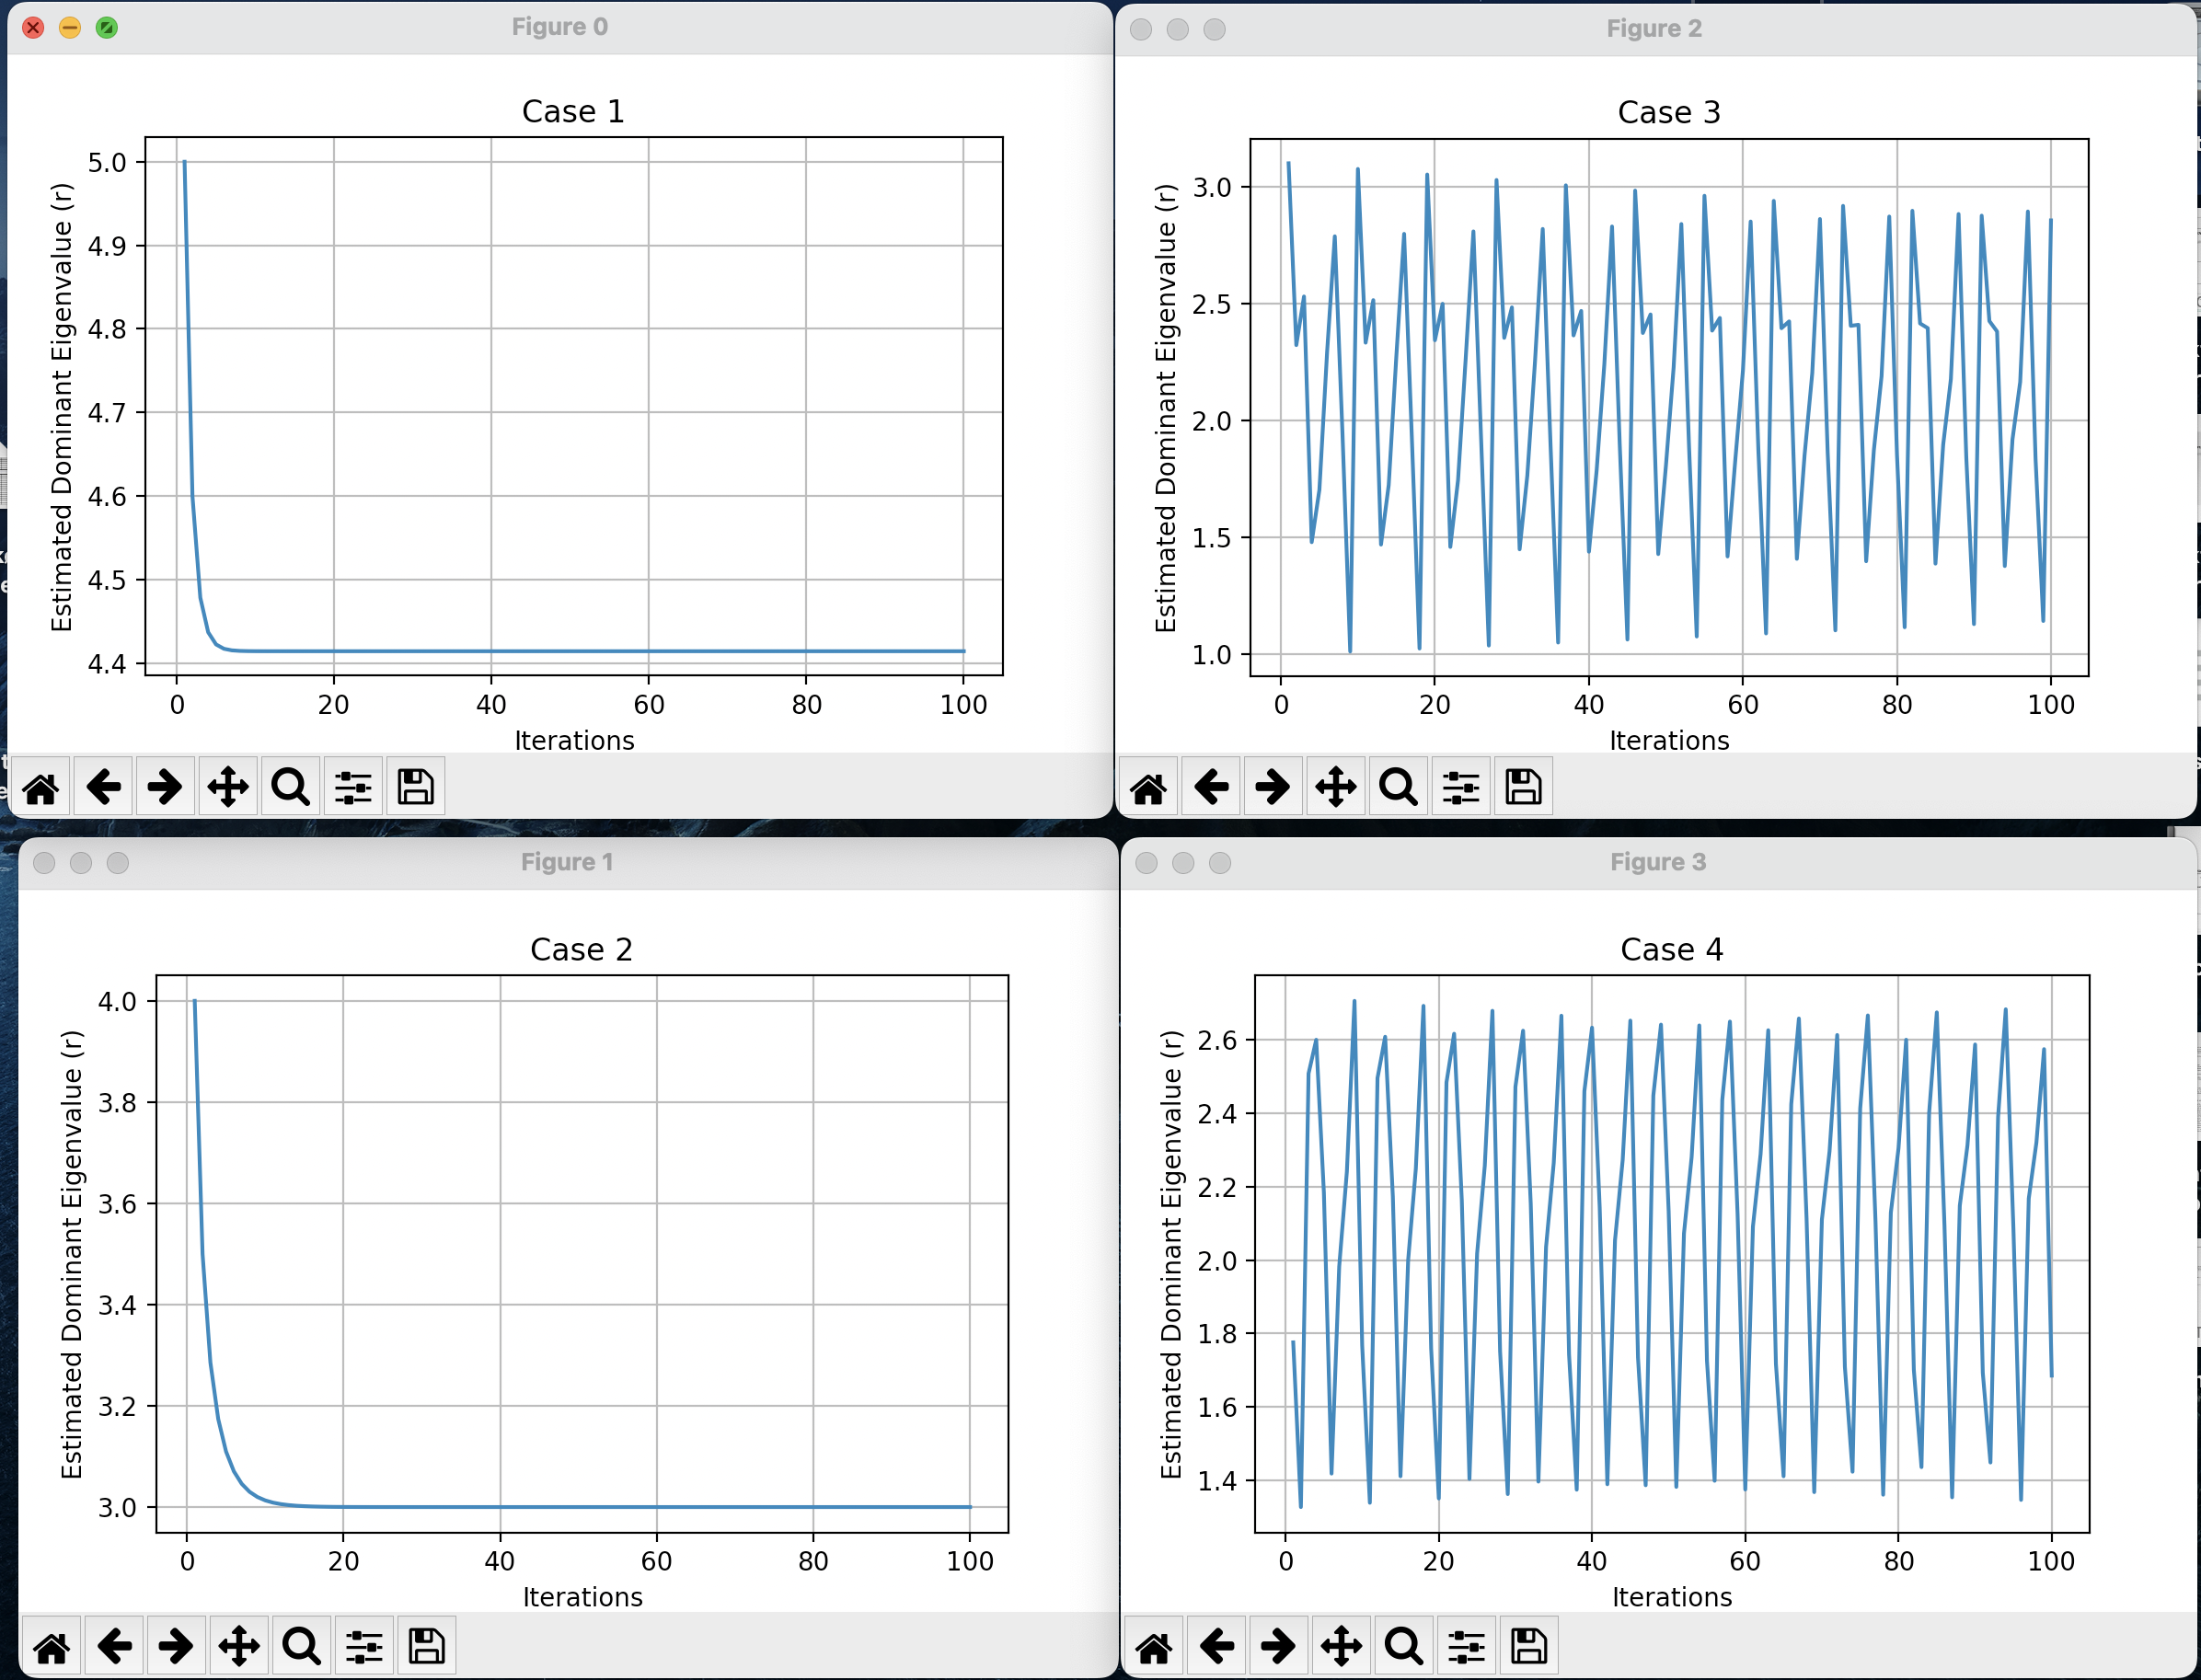
\includegraphics[scale=0.41]{p2.png}
\end{center}
\textbf{1. Case 1:}The plot starts high and gradually curves downwards. This indicates that the method is on a trajectory towards convergence. Given that the matrix is real and symmetric, the eigenvalue should eventually stabilize if more iterations are allowed.
\\
\\
\textbf{2. Case 2:} Similarly, this also starts from a high point and curves downwards. Even though the matrix and initial vector are complex, the behavior appears to be similar to Case 1. This suggests that the method is capable of handling complex numbers without significant difficulties in this specific case.
\\
\\
\textbf{3. Case 3:} The behavior here is notably different: the plot appears to oscillate, resembling an interference pattern. This suggests that the method is not converging. The eigenvalues of this matrix are probably complex or closely spaced, making it difficult for the power method to converge to a single dominant eigenvalue.
\\
\\
\textbf{4. Case 4:} Much like Case 3, this also shows an oscillatory behavior. The fact that both the matrix and the initial vector are complex might be causing these fluctuations, indicating a lack of convergence.
\end{document}
\endinput
%%
%% End of file `sample-authordraft.tex'.
